% !TEX encoding = UTF-8 Unicode
\documentclass[18pt,twoside]{extbook}


\usepackage{tikz}


%\PreviewEnvironment[]{pgfpicture}



\usetikzlibrary{calc}

\usetikzlibrary{positioning}

\usepackage{tcolorbox}

\tcbuselibrary{skins}




\usepackage{fontspec,xunicode}

\setmainfont{Open Sans Condensed Light}



\def \guatemala {10}
\def \altaVerapaz {21}
\def \bajaVerapaz {0.3}
\def \elProgreso {11.33}
\def \peten {9}
\def \izabal{1}
\def \zacapa {25}
\def \chiquimula {0.01}
\def \jalapa {3}
\def \jutiapa {7.7}
\def \santaRosa {4}
\def \sacatepequez{15.2}
\def \quiche {1.35}
\def \solola {37}
\def \totonicapan {17}
\def \quetzaltenango {8.9}
\def \sanMarcos {5.3}
\def \huehuetenango {1.3}
\def \retalhuleu {4}
\def \suchitepequez{19.2}
\def \chimaltenango {0.98}
\def \escuintla {6.7}
\definecolor{color1}{RGB}{0,0,128}
\definecolor{color2}{RGB}{100,100,220}

\usepackage[active,tightpage,xetex]{preview}


\PreviewEnvironment[]{tikzpicture}
\setlength\PreviewBorder{0pt}
\thispagestyle{empty}
\def \guatemala {10}
\def \altaVerapaz {21}
\def \bajaVerapaz {0.3}
\def \elProgreso {11.33}
\def \peten {9}
\def \izabal{1}
\def \zacapa {25}
\def \chiquimula {0.01}
\def \jalapa {3}
\def \jutiapa {7.7}
\def \santaRosa {4}
\def \sacatepequez{15.2}
\def \quiche {1.35}
\def \solola {37}
\def \totonicapan {17}
\def \quetzaltenango {8.9}
\def \sanMarcos {5.3}
\def \huehuetenango {1.3}
\def \retalhuleu {4}
\def \suchitepequez{19.2}
\def \chimaltenango {0.98}
\def \escuintla {6.7}
\begin{document}
\begin{tikzpicture}
\node[anchor=south west,inner sep=0] (image) at (0,0) {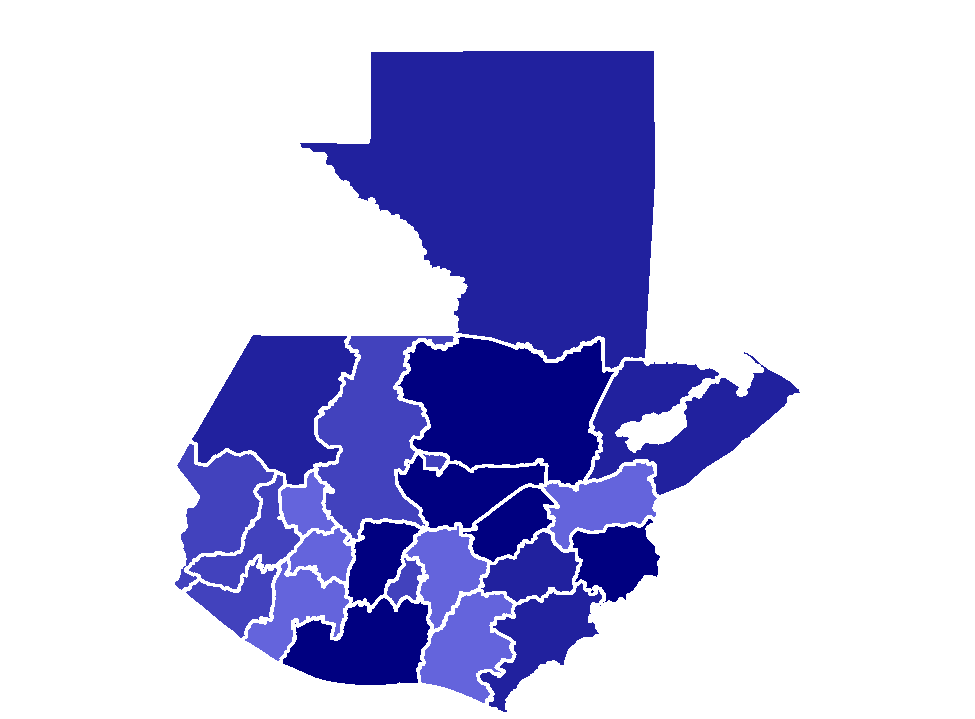
\includegraphics{mapa}};
\begin{scope}[x={(image.south east)},y={(image.north west)}]
%\draw[help lines,xstep=.1,ystep=.1] (0,0) grid (1,1);
%\foreach \x in {0,1,...,9} { \node [anchor=north] at (\x/10,0) {0.\x}; }
%\foreach \y in {0,1,...,9} { \node [anchor=east] at (0,\y/10) {0.\y}; }

%\node[text width=8cm, draw] at (0.6,1.02) {\Large AQUÍ VA LA ESCALA DE COLORES};

% ##############GUATEMALA############################## %
%\draw [ gray] (0.46,0.2) -- (0.46,0.99);
%\filldraw [gray] (0.46,0.2) circle (1.2pt);
%\draw [ gray] (0.46,0.99) -- (0.73,0.99);
%\node[text width=1.5cm, draw] at (0.83,0.99) {Guatemala \\ \guatemala };

\draw [ gray] (0.46,0.2) -- (0.46,0.03);
\filldraw [gray] (0.46,0.2) circle (1.2pt);
\draw [ gray] (0.46,0.03) -- (0.73,0.03);
\node[text width=1.5cm, draw] at (0.835,0.03) {Guatemala  \\ \guatemala };


% ###############ALTA VERAPAZ############################## %
\draw [ gray] (0.5,0.4) -- (0.5,0.9);
\filldraw [gray] (0.5,0.4) circle (1.2pt);
\draw [ gray] (0.4989,0.9) -- (0.85,0.9);
\node[text width=1.4cm, draw] at (0.95,0.9) {AltaVerapaz \\ \altaVerapaz };





% ###############BAJA VERAPAZ############################## %
\draw [ gray] (0.525,0.33) -- (0.525,0.83);
\filldraw [gray] (0.525,0.33) circle (1.2pt);
\draw [ gray] (0.525,0.83) -- (0.73,0.83);
\node[text width=1.5cm, draw] at (0.835,0.83) {Baja Verapaz \\ \bajaVerapaz };

%#############EL PROGRESO################################# %
\draw [ gray] (0.55,0.28) -- (0.55,0.76);
\filldraw [gray] (0.55,0.28) circle (1.2pt);
\draw [ gray] (0.55,0.76) -- (0.85,0.76);
\node[text width=1.4cm, draw] at (0.95,0.76) {El Progreso \\  \elProgreso };


% ###############PETEN############################## %
\draw [ gray] (0.58,0.65) -- (0.58,0.69);
\filldraw [gray] (0.58,0.65) circle (1.2pt);
\draw [ gray] (0.58,0.69) -- (0.73,0.69);
\node[text width=1.5cm, draw] at (0.835,0.69) {Petén \\  \peten };

%#############IZABAL################################# %
\draw [ gray] (0.64,0.45) -- (0.64,0.62);
\filldraw [gray] (0.64,0.45) circle (1.2pt);
\draw [ gray] (0.6389,0.62) -- (0.85,0.62);
\node[text width=1.4cm, draw] at (0.95,0.62) {Izabal \\  \izabal };



%#############ZACAPA################################# %
\filldraw [gray] (0.59,0.29) circle (1.2pt);
\draw [ gray] (0.59,0.29) -- (0.59,0.39);
\draw [ gray] (0.59,0.39) -- (0.85,0.39);
\node[text width=1.4cm, draw] at (0.95,0.39) {Zacapa \\ \zacapa };


%#############CHIQUIMULA################################# %
\filldraw [gray] (0.62,0.24) circle (1.2pt);
\draw [ gray] (0.62,0.24) -- (0.62,0.32);
\draw [ gray] (0.62,0.32) -- (0.73,0.32);
\node[text width=1.5cm, draw] at (0.835,0.32) {Chiquimula \\  \zacapa };

%#############JALAPA################################# %
\filldraw [gray] (0.55,0.20) circle (1.2pt);
\draw [ gray] (0.65,0.20) -- (0.65,0.25);
\draw [ gray] (0.65,0.25) -- (0.85,0.25);
\draw [ gray] (0.55,0.20) -- (0.65,0.20);
\node[text width=1.4cm, draw] at (0.95,0.25) {Jalapa \\  \jalapa };

%#############JUTIAPA################################# %
\filldraw [gray] (0.57,0.15) circle (1.2pt);
\draw [ gray] (0.57,0.15) -- (0.69,0.15);
\draw [ gray] (0.69,0.15) -- (0.69,0.18);
\draw [ gray] (0.69,0.18) -- (0.73,0.18);
\node[text width=1.5cm, draw] at (0.835,0.18) {Jutiapa \\  \jutiapa };

%#############SANTA ROSA################################# %
\filldraw [gray] (0.48,0.11) circle (1.2pt);
\draw [ gray] (0.48,0.11) -- (0.85,0.11);
%\draw [ gray] (0.48,0.11) -- (0.48,0.11);
\node[text width=1.4cm, draw] at (0.95,0.11) {Santa Rosa \\  \santaRosa };


% ###############SACATEPEQUEZ############################## %
%\draw [ gray] (0.42,0.2) -- (0.42,0.99);
%\filldraw [gray] (0.42,0.2) circle (1.2pt);
%\draw [ gray] (0.42,0.99) -- (0.20,0.99);
%\node[align=right, text width=1.5cm, draw] at (0.10,0.99) {Sacatepéquez \\ \sacatepequez };

\draw [ gray] (0.42,0.2) -- (0.42,0.03);
\filldraw [gray] (0.42,0.2) circle (1.2pt);
\draw [ gray] (0.42,0.03) -- (0.00,0.03);
\node[align=right, text width=1.5cm, draw] at (-0.10,0.03) {Sacatepéquez \\ \sacatepequez };

% ###############QUICHE############################## %
\draw [ gray] (0.39,0.4) -- (0.39,0.9);
\filldraw [gray] (0.39,0.4) circle (1.2pt);
\draw [ gray] (0.39,0.9) -- (0.00,0.9);
\node[align=right, text width=1.5cm, draw] at (-0.07,0.9) {Quiché \\ \quiche };


% ###############SOLOLÁ############################## %
\draw [ gray] (0.34,0.23) -- (0.34,0.83);
\filldraw [gray] (0.34,0.23) circle (1.2pt);
\draw [ gray] (0.34,0.83) -- (0.16,0.83);
\node[align=right,text width=1.5cm, draw] at (0.09,0.83) {Sololá \\ \solola };

% ###############TOTONICAPAN############################## %
\draw [ gray] (0.31,0.29) -- (0.31,0.76);
\filldraw [gray] (0.31,0.29) circle (1.2pt);
\draw [ gray] (0.31,0.76) -- (0.00,0.76	);
\node[align=right,text width=1.5cm, draw] at (-0.10,0.76) {Totonicapán \\ \totonicapan };

% ###############QUETZALTENANGO############################## %
\draw [ gray] (0.28,0.26) -- (0.28,0.69);
\filldraw [gray] (0.28,0.26) circle (1.2pt);
\draw [ gray] (0.28,0.69) -- (0.16,0.69	);
\node[align=right,text width=1.5cm, draw] at (0.09,0.69) {Quetzaltenango \\ \quetzaltenango };




% ###############SAN MARCOS############################## %
\draw [ gray] (0.24,0.34) -- (0.24,0.62);
\filldraw [gray] (0.24,0.34) circle (1.2pt);
\draw [ gray] (0.24,0.62) -- (0.00,0.62	);
\node[align=right,text width=1.5cm, draw] at (-0.10,0.62) {San Marcos \\ \sanMarcos };


% ###############HUEHUETENANGO############################## %
\draw [ gray] (0.22,0.4) -- (0.22,0.55);
\filldraw [gray] (0.22,0.4) circle (1.2pt);
\draw [ gray] (0.22,0.55) -- (0.15,0.55	);
\node[align=right,text width=1.5cm, draw] at (0.09,0.55) {Huehuetenango \\ \huehuetenango };



% ###############ESCUINTLA############################## %
\draw [ gray] (0.32,0.12) -- (0.19,0.12);
\filldraw [gray] (0.32,0.12) circle (1.2pt);
\draw [ gray] (0.19,0.12) -- (0.19,0.17	);
\draw [ gray] (0.19,0.17) -- (0.00,0.17	);
\node[align=right,text width=1.5cm, draw] at (-0.10,0.17) {Escuintla \\ \escuintla };


% ###############CHIMALTENANGO############################## %
\draw [ gray] (0.38,0.22) -- (0.38,0.07);
\filldraw [gray] (0.38,0.22) circle (1.2pt);
\draw [ gray] (0.38,0.07) -- (0.17,0.07	);
\draw [ gray] (0.17,0.07) -- (0.17,0.10	);
\draw [ gray] (0.17,0.10) -- (0.15,0.10	);
\node[align=right,text width=1.5cm, draw] at (0.09,0.10) {Chimaltenango \\ \chimaltenango };

% ###############SUCHITEPEQUEZ############################## %
\draw [ gray] (0.22,0.17) -- (0.22,0.24);
\filldraw [gray] (0.31,0.17) circle (1.2pt);
\draw [ gray] (0.31,0.17) -- (0.22,0.17	);
\draw [ gray] (0.22,0.24) -- (0.15,0.24	);
\node[align=right,text width=1.5cm, draw] at (0.09,0.24) {Suchitepéquez \\ \suchitepequez };

% ###############RETALHULEU############################## %
\draw [ gray] (0.26,0.19) -- (0.26,0.31);
\filldraw [gray] (0.26,0.19) circle (1.2pt);
\draw [ gray] (0.26,0.31) -- (0.00,0.31	);
\node[align=right,text width=1.5cm, draw] at (-0.10,0.31) {Retalhuleu \\  \retalhuleu };

\node (label) at (0.53,0.98) {
	
\includegraphics{barraColor.pdf}
	};
\node[align=right,text width=3cm, draw, color=gray] at (0.32,0.98) {Valores más pequeños};
\node[align=left,text width=3cm, draw, color=gray] at (0.74,0.98) {Valores más grandes};


\end{scope}


\end{tikzpicture}
\end{document}
